\documentclass[12pt,a4paper]{article}
\usepackage[english]{babel}
\usepackage[T1]{fontenc}
\usepackage[utf8x]{inputenc}
\usepackage{hyperref}
\usepackage{url}
\usepackage{graphicx}
\usepackage{float}
\usepackage{ctable}


\addtolength{\hoffset}{-1.5cm}
\addtolength{\marginparwidth}{-1.5cm}
\addtolength{\textwidth}{3cm}
\addtolength{\voffset}{-1cm}
\addtolength{\textheight}{2.5cm}
\setlength{\topmargin}{0cm}
\setlength{\headheight}{0cm}

\begin{document}

\title{Building application using Heroku and Salesforce\\ \linespread{2} \huge Instruction   }


\maketitle
\newpage
\tableofcontents
\newpage

\section{Introduction}
\subsection{Salesforce}
Salesforce is CRM software and enterprise ecosystem. The Salesforce customer portal provides customers the ability to track their own cases, includes a social networking plug-in that enables the user to join the conversation about their company on social networking websites, provides analytical tools and other services including email alert, Google search, and access to customers' entitlement and contracts.\cite{cos}
\subsection{Heroku}
Heroku is a cloud Platform-as-a-Service (PaaS) supporting several programming languages, that is used as a web application deployment model like Node, Ruby, PHP, Go, Scala, Python, Java, Clojure. \cite{wiki}
\subsubsection{Heroku Postgres}
Heroku Postgres is the Cloud database (DBaaS) service form Heroku based on PostgreSQL. Heroku Postgres provides features like continuous protection, rollback and high availability and also forks, followers and dataclips.\cite{wiki}
\subsubsection{Heroku Connect}
Heroku Connect lets users to Heroku apps that can easily integrate with Salesforce deployments at scale. This is done by having a seamless data synchronization between Heroku Postgres databases and Salesforce organizations.\cite{wiki}
\section{Preinstallation}
Before you start main configurations, you should install following programs:

\begin{itemize}
\item Git: \url{https://git-scm.com/downloads} and account on GitHub
\item Console: ex. \url{http://cmder.net/}
\item IDE: ex. IntelliJ \url{https://www.jetbrains.com/idea/#chooseYourEdition}
\item Python 3.6.0: \url{https://www.python.org/downloads/} and pip \url{https://pip.pypa.io/en/stable/installing/} Remember to add Python to path(during installation it will ask you about it).
\item Apache Ant: instruction\\ \url{https://www.mkyong.com/ant/how-to-install-apache-ant-on-windows/} 



\end{itemize}

\section{Salesforce}
\subsection{Sign Up to Salesforce}
To sign up open following link: \url{https://developer.salesforce.com/signup}.
Fill the gaps and select 'Developer' in 'Role' field.
\subsection{Network access configuration}
To successfully deployment it is needed to configure network access.
\begin{figure}[H]
	\centering
	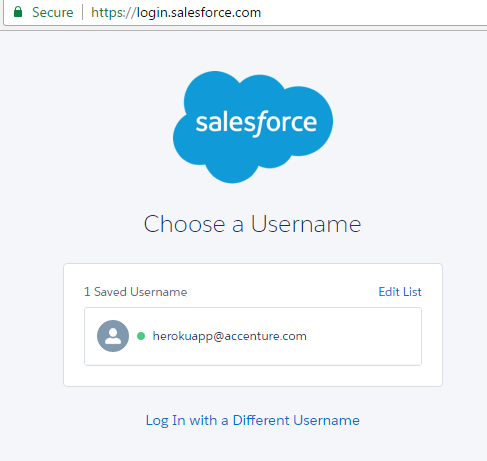
\includegraphics{images/connect5.PNG}
	\caption{Logging into Salesforce.}
	\label{fig:log}
\end{figure}
To do that it is needed to know the user’s IP address. IP can be checked using site: \url{https://www.whatismyip.com/}.
Once you know the IP address click 'setup' section. In the quick find search for network access and click on it.  

\begin{figure}[H]
	\centering
	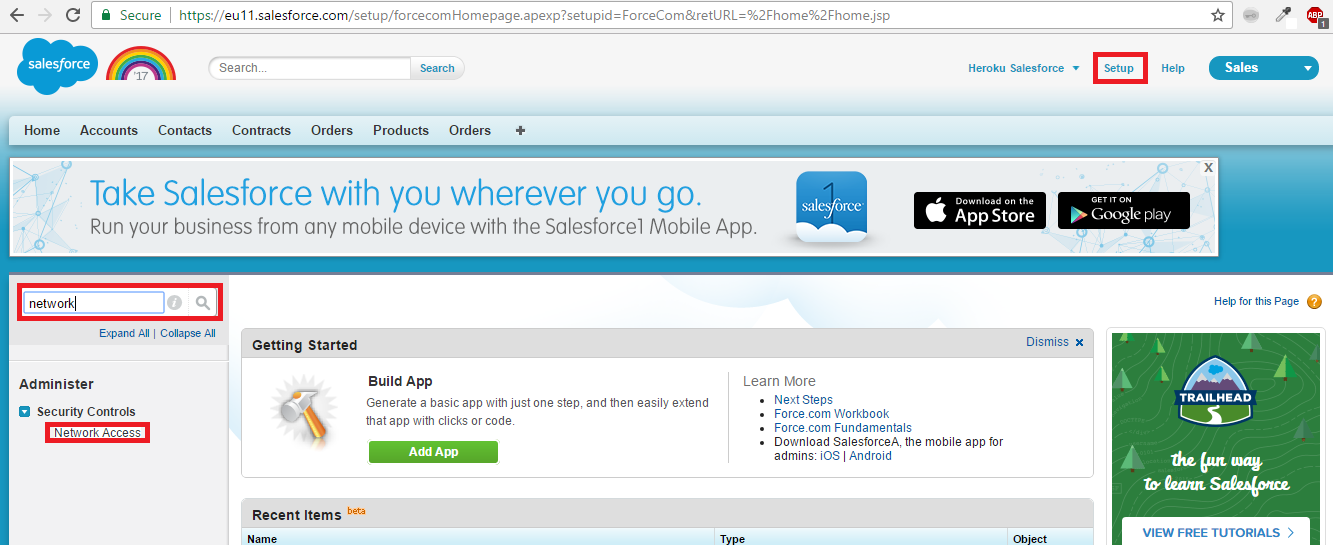
\includegraphics[width = 1 \textwidth]{images/network.PNG}
	\caption{Setup.}
	\label{fig:setup}
\end{figure}

Click 'New'. Paste IP of yours in 'Start IP Address' section. In 'End IP address' add the same IP with some extra range.

\begin{figure}[H]
	\centering
	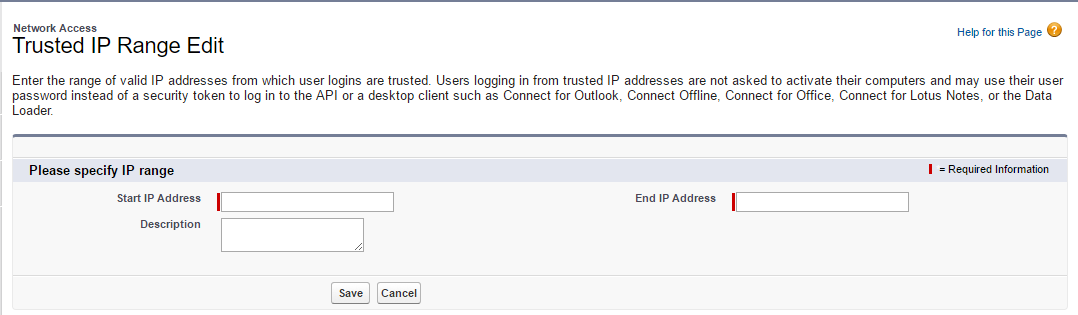
\includegraphics[width = 1 \textwidth]{images/network2.PNG}
	\caption{Setup network access.}
	\label{fig:setupp}
\end{figure}

\subsection{Salesforce deployment using Ant}
Download repository with command:\\
\begin{tabular}{|l|}
	\hline
	git clone https://github.com/HerokuAcc/pizzaman.git \textit{YourRepoPath}\\
	\hline
\end{tabular}\\

In order to deploy prepared Salesforce configurations use downloaded repository. Open console, move to repository and 'salesforce' file using commands:\\

\begin{tabular}{|l|}
	\hline
	cd \textit{YourRepoPath}\\
	cd salesforce\\
	\hline
\end{tabular}\\

Edit 'build.properties\_example' change username and password to one you use for Salesforce and save file as 'build.properties'
Then write in your console command for Ant:

\begin{tabular}{|l|}
	\hline
	ant deploy\\
	\hline
\end{tabular}\\


This will deploy custom fields, objects and ProcessBuilder to your  Salesforce.\\
To activate workflows go to 'Setup', in 'Quick find' type 'process builder' and then click on it. Activate both process build's by clicking on the name of processes and 'Activate' button.
\begin{figure}[H]
	\centering
	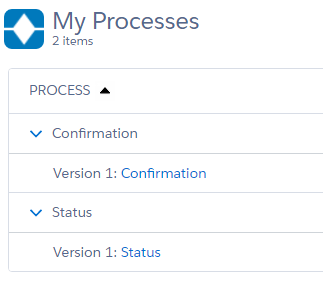
\includegraphics{images/process.PNG}
	\caption{Finding process.}
	\label{fig:process}
\end{figure}
\begin{figure}[H]
	\centering
	
\includegraphics{images/process2.PNG}
	\caption{Activate button.}
	\label{fig:processs}
\end{figure}

Copy everything from pizza.txt file in salesforce folder and paste it into Anonymous Apex through developer console in Salesforce.
To do that find Developer Console, use hot key CTRL+E and click 'Execute' button.

\begin{figure}[H]
	\centering
	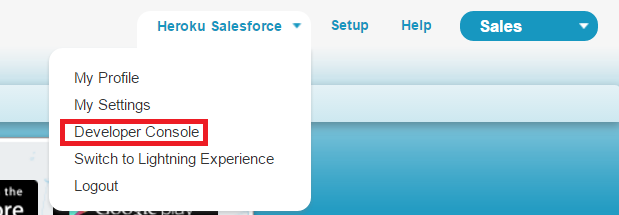
\includegraphics[width=1\textwidth]{images/deploy1.PNG}
	\caption{Developer Console.}
	\label{fig:console}
\end{figure}

\begin{figure}[H]
	\centering
	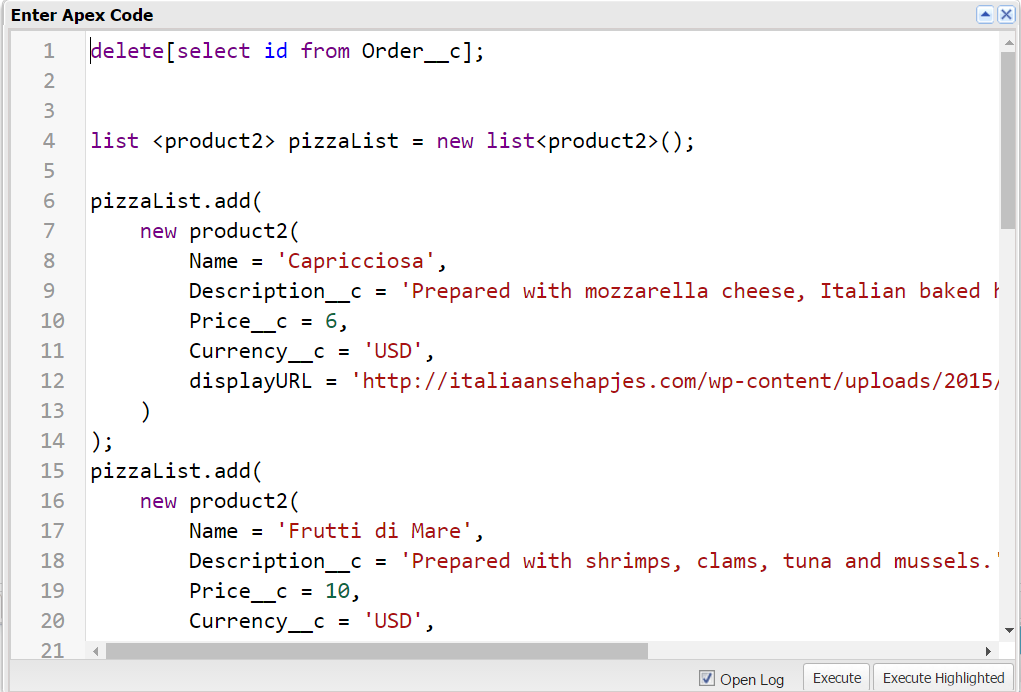
\includegraphics[width=1\textwidth]{images/deploy2.PNG}
	\caption{Anonymous Apex.}
	\label{fig:apex}
\end{figure}

\subsection{Creating tab}

In order to have easier access to custom object you have to create tab. To do that, open 'Setup', an in 'Quick find' type 'tab'. Click on 'Tab'.

\begin{figure}[H]
	\centering
	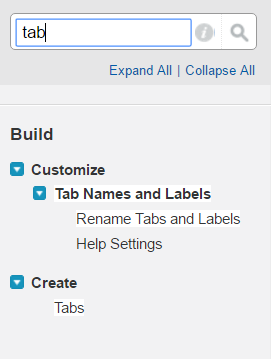
\includegraphics{images/tab.PNG}
	\caption{Finding a tab.}
	\label{fig:tab}
\end{figure}

Then click 'New' button and choose an object you want. Then click 'Next' all the time. In the end click 'Save'.

\begin{figure}[H]
	\centering
	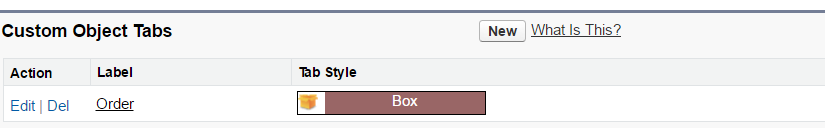
\includegraphics{images/create.PNG}
	\caption{Creating new tab.}
	\label{fig:tabb}
\end{figure}

\begin{figure}[H]
	\centering
	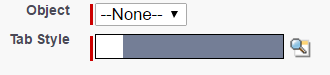
\includegraphics{images/tabobj.PNG}
	\caption{Selecting an object.}
	\label{fig:tabbb}
\end{figure}
 
\section{Heroku}
\subsection{Sign Up to Heroku}
Create account in Heroku: \url{https://signup.heroku.com/login}. Select development language to Python. 
Now you can create your own app according to steps below:

\begin{enumerate}
	\item Click 'New' button and select 'Create new app'
	\item Name your app. Remember that name must be unique.
	\item Choose Runtime Selection to Europe. 
\end{enumerate}

\subsection{Connect to Git}
To connect Heroku with Git click on menu and then select 'Deploy'. In 'Deployment method' choose GitHub.
\begin{figure}[H]
	\centering
	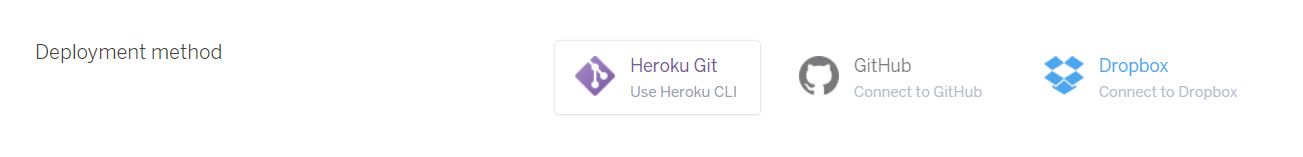
\includegraphics[width = 1 \textwidth]{images/git.PNG}
	\caption{Connect Heroku to GitHub}
	\label{fig:git}
\end{figure}

Next step is selecting repository.

\begin{figure}[H]
	\centering
	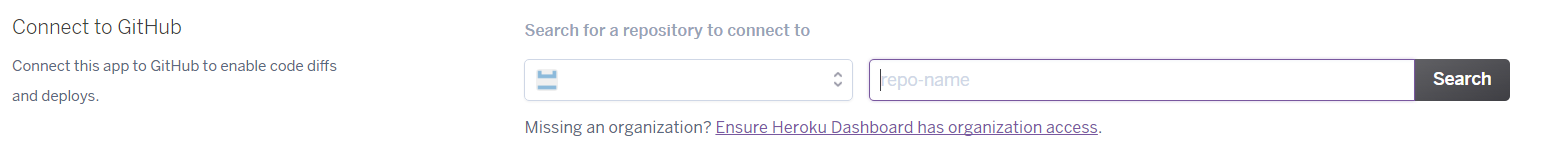
\includegraphics[width = 1 \textwidth]{images/git2.PNG}
	\caption{Connect Heroku to GitHub - selecting repository}
	\label{fig:git2}
\end{figure}


\subsection{Postgres}
In order to open your app, click on menu and then select 'Dashboard'.\\

\begin{figure}[H]
\centering
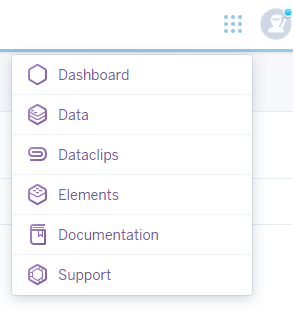
\includegraphics{images/dashboard.PNG}
\caption{Heroku menu}
\label{fig:menu}
\end{figure}
After that, choose your app and select 'Resources' button.
\begin{figure}[H]
	\centering
	
\includegraphics{images/nav.PNG}
	\caption{Heroku options}
	\label{fig:nav}
\end{figure}


To add Postgres add-on, type 'Postgres' word and click on 'Heroku Postgres'. 
\begin{figure}[H]
	\centering
	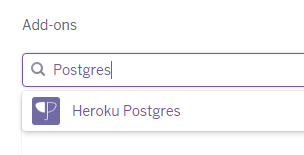
\includegraphics{images/addon.PNG}
	\caption{Heroku add-ons}
	\label{fig:addon}
\end{figure}

The last step is to confirm configurations by clicking 'Provision'.
\begin{figure}[H]
	\centering
	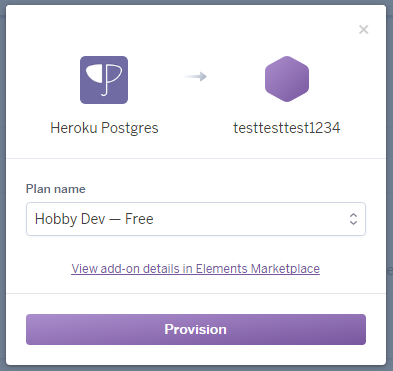
\includegraphics{images/postgres1.PNG}
	\caption{Confirmation}
	\label{fig:addonn}
\end{figure}

\subsection{Heroku Connect}
In order to connect Heroku and Salesforce, Heroku Connect is needed. Follow the steps to configure it:
\begin{enumerate}
	
 \item As a Postgres, Heroku Connect is an add-on. For this reason, in case shown on Figure \ref{fig:addon}, you can type 'Connect' word and click 'Heroku Connect'. Then click 'Provision'.\\
Now you have Heroku Connect avaliable.
\begin{figure}[H]
	\centering
	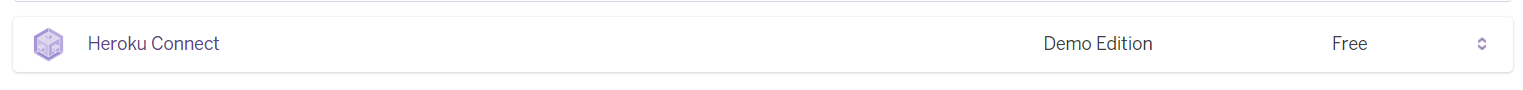
\includegraphics[width=1\textwidth]{images/connect1.PNG}
	\caption{Avaliable Heroku Connect.}
	\label{fig:cona}
\end{figure}

\item Click on 'Setup connection' button.
\begin{figure}[H]
	\centering
	
\includegraphics{images/connect2.PNG}
	\caption{Setup connection.}
	\label{fig:conb}
\end{figure}

\item If everything is up-to-date and look like it is shown on Figure \ref{fig:conc}, click 'Next' button.

\begin{figure}[H]
	\centering
	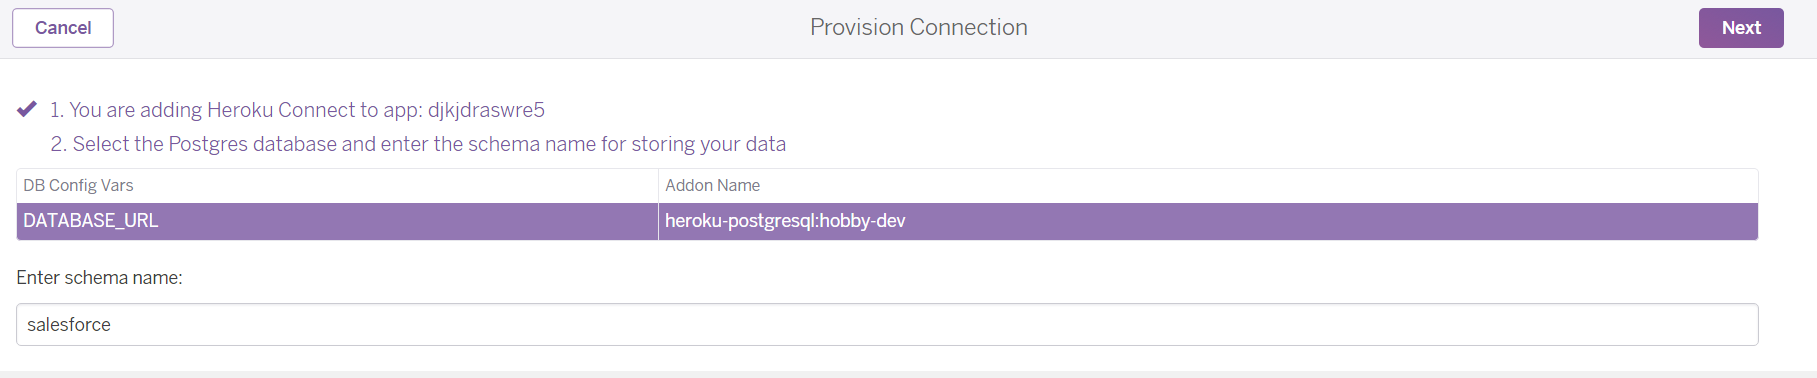
\includegraphics[width=1\textwidth]{images/connect3.PNG}
	\caption{Setup.}
	\label{fig:conc}
\end{figure}

\item Click 'Authorize' button with settings as shown on Figure \ref{fig:cond}.

\begin{figure}[H]
	\centering
	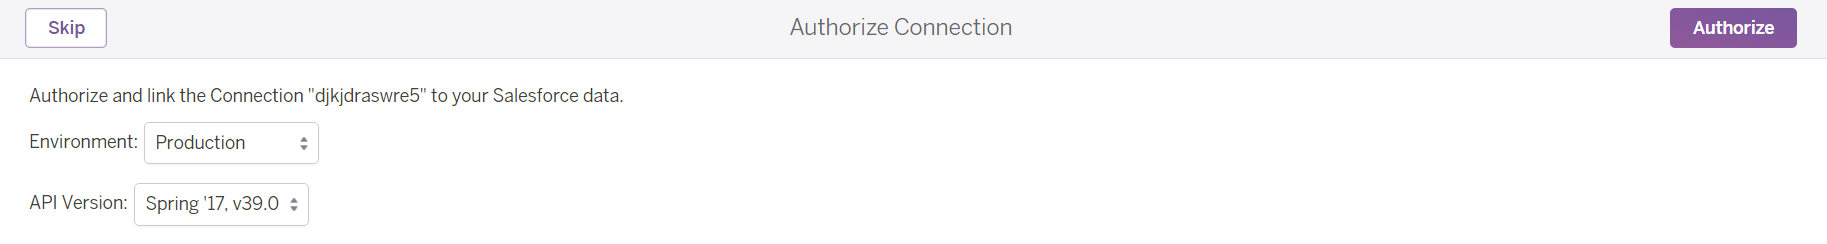
\includegraphics[width=1\textwidth]{images/connect4.PNG}
	\caption{Authorization.}
	\label{fig:cond}
\end{figure}

\item Log into your Salesforce account, ex. Figure \ref{fig:cone}.

\begin{figure}[H]
	\centering
	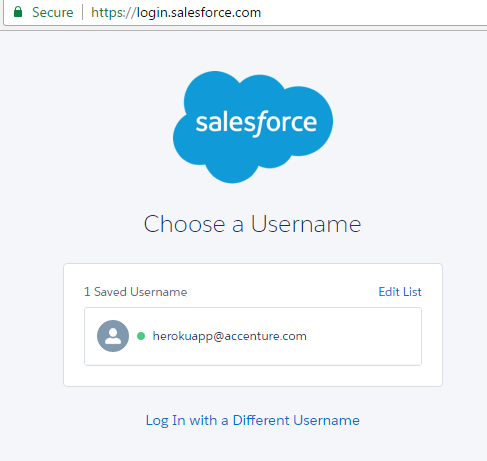
\includegraphics{images/connect5.PNG}
	\caption{Logging in to Salesforce}
	\label{fig:cone}
\end{figure}

\item Click 'Create mapping' button. Becouse of that, you can choose objects and fields in Salesforce you want to have connected with Heroku.
\begin{figure}[H]
	\centering
	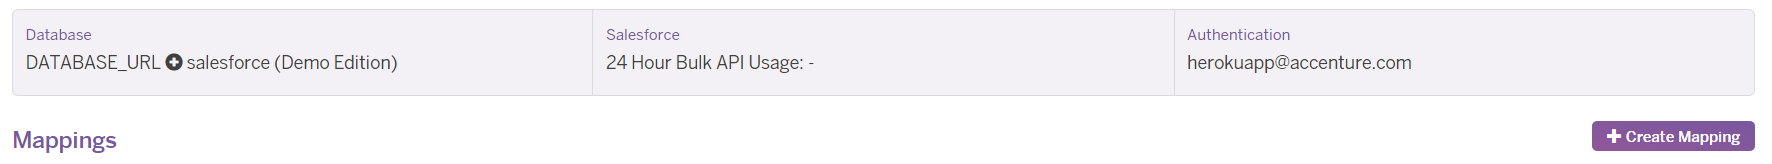
\includegraphics[width=1\textwidth]{images/connect6.PNG}
	\caption{Mapping}
	\label{fig:conf}
\end{figure}

\item Find and click object you want to map.
\begin{figure}[H]
	\centering
	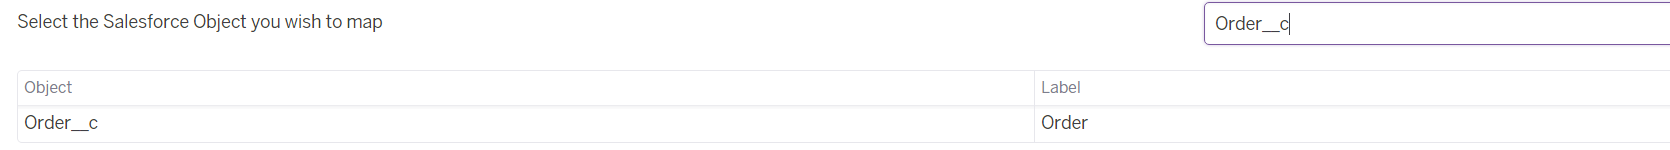
\includegraphics[width=1\textwidth]{images/connect7.PNG}
	\caption{Mapping-finding needed object.}
	\label{fig:cong}
\end{figure}

\item Set connection way. You have possibility to set if you want to listen for Salesforce updates or/and write updates from Heroku to Salesforce. You can also set synchronization frequency. 
\begin{figure}[H]
	\centering
	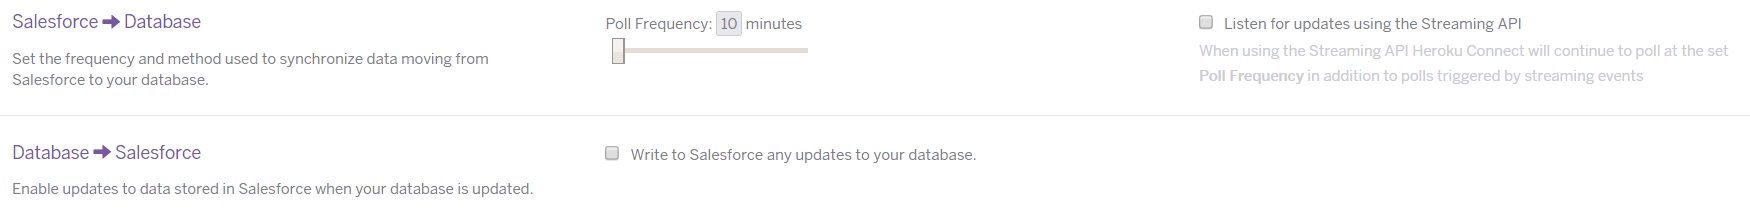
\includegraphics[width=1\textwidth]{images/connect8.PNG}
	\caption{Setting connection way.}
	\label{fig:conh}
\end{figure}

\item Select field you want to map. 

\begin{figure}[H]
	\centering
	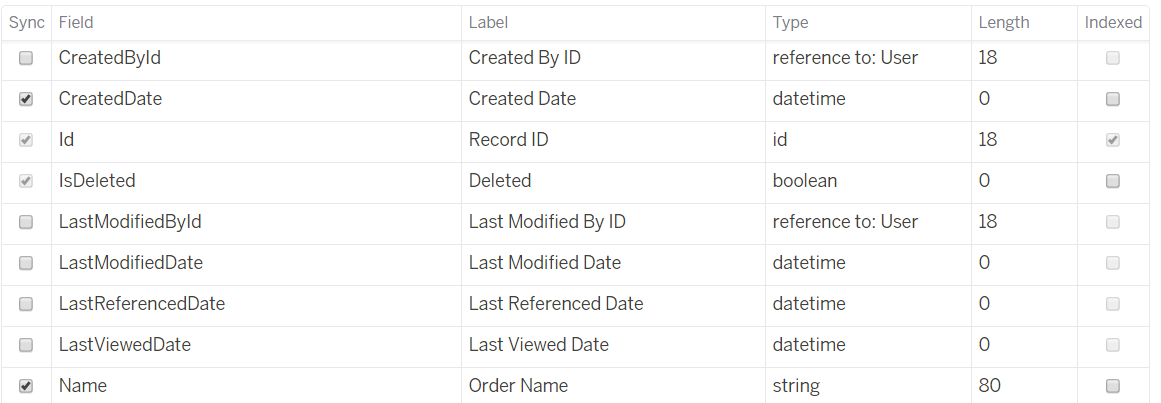
\includegraphics[width=1\textwidth]{images/connect9.PNG}
	\caption{Setting-selecting needed fields.}
	\label{fig:coni}
\end{figure}

Now your mapping is placed on mapping list in Heroku Connection bookmark. 

\begin{figure}[H]
	\centering
	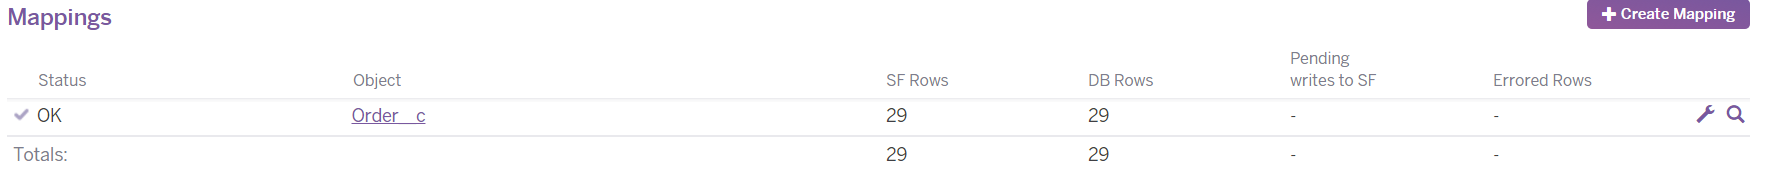
\includegraphics[width=1\textwidth]{images/connect10.PNG}
	\caption{Mapping effect.}
	\label{fig:conj}
\end{figure}

\end{enumerate} 

List of objects and fields you must map and cofigurations you must check:\\
\begin{tabular}{|c|c|c|}
	\hline
	Object&Field&Configurations\\ 
	\specialrule{.2em}{.1em}{.1em} 
	Product2&CreatedDate&none, frequency: 10 min\\
	\hline
	Product2&Currency\_\_c &none, frequency: 10 min\\
	\hline
	Product2&Descripion\_\_c &none, frequency: 10 min\\
	\hline
	Product2&DisplayUrl& none, frequency: 10 min\\
	\hline
	Product2&Id&none, frequency: 10 min\\
	\hline
	Product2&IsDeleted& none, frequency: 10 min\\
	\hline		
	Product2&Name& none, frequency: 10 min\\
	\hline
	Product2&Price\_\_c& none, frequency: 10 min\\
	\hline			
	Product2&SystemModstamp&none, frequency: 10 min\\
	\specialrule{.2em}{.1em}{.1em}
	Order\_\_c& CreatedDate&Write to Salesforce , frequency: 10 min\\ 
	\hline
	Order\_\_c&Id&Write to Salesforce , frequency: 10 min\\ 
	\hline
	Order\_\_c&IdDeleted&Write to Salesforce , frequency: 10 min\\ 
	\hline
	Order\_\_c&Name&Write to Salesforce , frequency: 10 min\\ 
	\hline
	Order\_\_c&SystemModstamp&Write to Salesforce , frequency: 10 min\\ 
	\hline
Order\_\_ c&cst\_city\_\_c&Write to Salesforce , frequency: 10 min\\ 
	\hline
Order\_\_c&cst\_email\_\_c&Write to Salesforce , frequency: 10 min\\ 
	\hline			
	Order\_\_c&cst\_name\_\_c&Write to Salesforce , frequency: 10 min\\ 
	\hline	
	Order\_\_c&cst\_phone\_\_c&Write to Salesforce , frequency: 10 min\\ 
	\hline	
	Order\_\_c&cst\_postal\_code\_\_c&Write to Salesforce , frequency: 10 min\\ 
	\hline	
	Order\_\_c&cst\_street\_\_c&Write to Salesforce , frequency: 10 min\\ 
	\hline		
	Order\_\_c&cst\_surname\_\_c&Write to Salesforce , frequency: 10 min\\ 
	\hline	
	Order\_\_c&cst\_productID\_\_c&Write to Salesforce , frequency: 10 min\\ 
	\hline	
	Order\_\_c&cst\_status\_\_c&Write to Salesforce , frequency: 10 min\\ 
	\hline						
				
\end{tabular}

\section{DATABASES settings}
To use prepared configurations, open project downloaded from GitHub. Open \textit{gettingstarted} directory. Next, open \textit{settings.py} file. Here is \textit{DATABASES} attribute you insert your data.  

\begin{figure}[H]
	\centering
	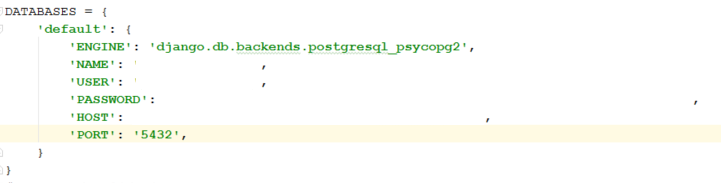
\includegraphics[width=1\textwidth]{images/databases.PNG}
	\caption{DATABASES method.}
	\label{fig:data}
\end{figure}

To get information about data you want insert, log into Heroku. Open your app, then 'Resources' and Postgres. Find 'Administration', 'Database Credintals' and click 'View Credintals' button. Here are needed data.

\begin{figure}[H]
	\centering
	
\includegraphics[width=1\textwidth]{images/admin.PNG}
	\caption{Administartion.}
	\label{fig:ad}
\end{figure}

\begin{figure}[H]
	\centering
	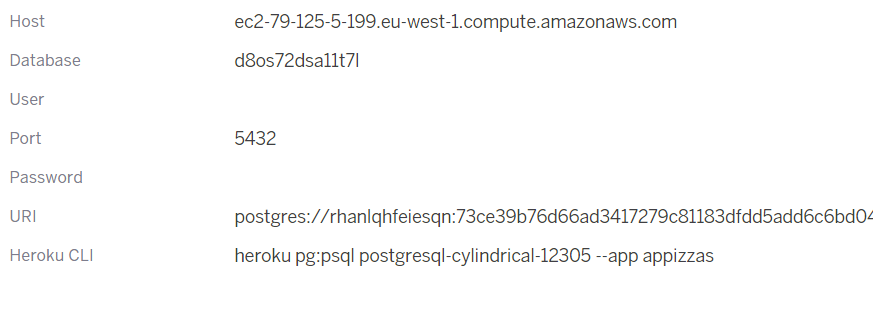
\includegraphics[width=1\textwidth]{images/datas.PNG}
	\caption{Administration data.}
	\label{fig:da}
\end{figure}


\section{Code deployment}
In order to open app, you can do it by Heroku or using commands. \\
\subsection{By Heroku}
Log into Heroku and open 'Deploy'. Find 'Automatic Deploys' and set configurations as shown on Figure\ref{fig:dep}. Then click on 'Enable Automatic Deploys'.

\begin{figure}[H]
	\centering
	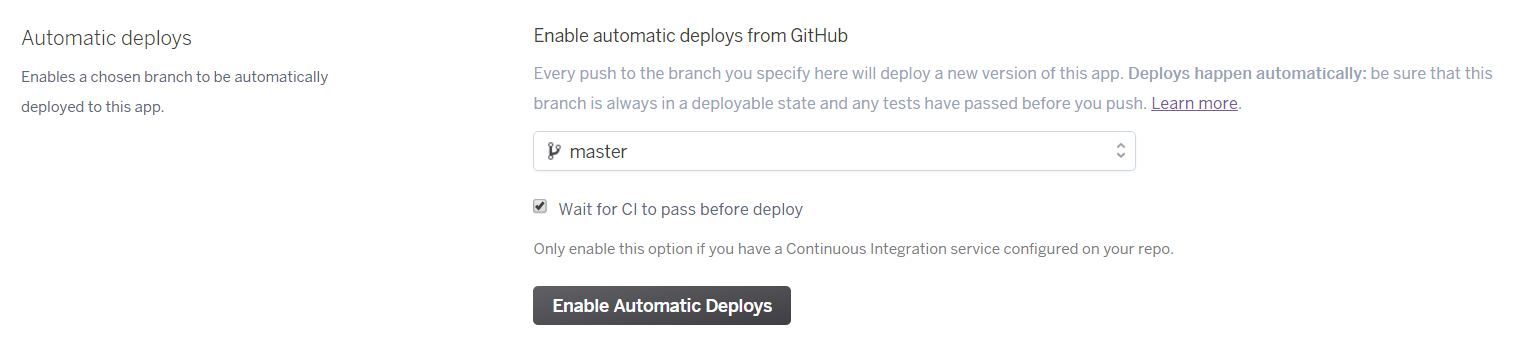
\includegraphics[width=1\textwidth]{images/deploy.PNG}
	\caption{Deploying code.}
	\label{fig:dep}
\end{figure}

\subsection{Using commands}
To open app in local host type in console following commands:\\
\begin{tabular}{|l|}
	\hline
	cd..\\
	heroku login\\
	heroku git:remote -a \textit{YourAppName}\\
	git commit -am "Deploying app for the first time"\\
	git push heroku origin\\
	heroku open\\
	\hline
\end{tabular}\\

\begin{thebibliography}{bib}
	\bibitem{cos} 
	 Rao, Leena. 
	\textit{Everything You Need To Know About Salesforce's Service Cloud 2}. 
	TechCrunch, Retrieved. September 8, 2009.
	 
	
	\bibitem{wiki}
	Wikipedia
	\\\texttt{https://en.wikipedia.org/wiki/Heroku}
	
\end{thebibliography}


\end{document}
